% Options for packages loaded elsewhere
\PassOptionsToPackage{unicode}{hyperref}
\PassOptionsToPackage{hyphens}{url}
\documentclass[
  twocolumn]{article}
\usepackage{xcolor}
\usepackage[a4paper, margin=1.5cm]{geometry}
\usepackage{amsmath,amssymb}
\setcounter{secnumdepth}{-\maxdimen} % remove section numbering
\usepackage{iftex}
\ifPDFTeX
  \usepackage[T1]{fontenc}
  \usepackage[utf8]{inputenc}
  \usepackage{textcomp} % provide euro and other symbols
\else % if luatex or xetex
  \usepackage{unicode-math} % this also loads fontspec
  \defaultfontfeatures{Scale=MatchLowercase}
  \defaultfontfeatures[\rmfamily]{Ligatures=TeX,Scale=1}
\fi
\usepackage{lmodern}
\ifPDFTeX\else
  % xetex/luatex font selection
\fi
% Use upquote if available, for straight quotes in verbatim environments
\IfFileExists{upquote.sty}{\usepackage{upquote}}{}
\IfFileExists{microtype.sty}{% use microtype if available
  \usepackage[]{microtype}
  \UseMicrotypeSet[protrusion]{basicmath} % disable protrusion for tt fonts
}{}
\makeatletter
\@ifundefined{KOMAClassName}{% if non-KOMA class
  \IfFileExists{parskip.sty}{%
    \usepackage{parskip}
  }{% else
    \setlength{\parindent}{0pt}
    \setlength{\parskip}{6pt plus 2pt minus 1pt}}
}{% if KOMA class
  \KOMAoptions{parskip=half}}
\makeatother
\usepackage{longtable,booktabs,array}
\usepackage{calc} % for calculating minipage widths
% Correct order of tables after \paragraph or \subparagraph
\usepackage{etoolbox}
\makeatletter
\patchcmd\longtable{\par}{\if@noskipsec\mbox{}\fi\par}{}{}
\makeatother
% Allow footnotes in longtable head/foot
\IfFileExists{footnotehyper.sty}{\usepackage{footnotehyper}}{\usepackage{footnote}}
\makesavenoteenv{longtable}
\usepackage{graphicx}
\makeatletter
\newsavebox\pandoc@box
\newcommand*\pandocbounded[1]{% scales image to fit in text height/width
  \sbox\pandoc@box{#1}%
  \Gscale@div\@tempa{\textheight}{\dimexpr\ht\pandoc@box+\dp\pandoc@box\relax}%
  \Gscale@div\@tempb{\linewidth}{\wd\pandoc@box}%
  \ifdim\@tempb\p@<\@tempa\p@\let\@tempa\@tempb\fi% select the smaller of both
  \ifdim\@tempa\p@<\p@\scalebox{\@tempa}{\usebox\pandoc@box}%
  \else\usebox{\pandoc@box}%
  \fi%
}
% Set default figure placement to htbp
\def\fps@figure{htbp}
\makeatother
\setlength{\emergencystretch}{3em} % prevent overfull lines
\providecommand{\tightlist}{%
  \setlength{\itemsep}{0pt}\setlength{\parskip}{0pt}}
\usepackage{bookmark}
\IfFileExists{xurl.sty}{\usepackage{xurl}}{} % add URL line breaks if available
\urlstyle{same}
\hypersetup{
  hidelinks,
  pdfcreator={LaTeX via pandoc}}

\author{}
\date{}

\begin{document}

\section{La Torre del Estratega: Cinco
Desafíos}\label{la-torre-del-estratega-cinco-desafuxedos}

\subsection{Introducción y Contexto}\label{introducciuxf3n-y-contexto}

Los personajes son un grupo de aventureros contratados para ascender la
enigmática Torre del Estratega, una estructura antigua llena de trampas,
secretos y guardianes creados para probar la capacidad de adaptación y
la astucia de quienes se atreven a desafiarla. Cada nivel presenta un
reto único, obligando a los PJ a estudiar a sus enemigos, ajustar su
equipo y aprovechar el entorno para sobrevivir.

\textbf{Este documento se basa en las reglas de D\&D5.}

\textbf{En esta partida, se puede volver atrás en el tiempo para
deshacer acciones.}

\textbf{Es conveniente usar relojes de arena para presionar a los
jugadores.}

\subsection{Encuentro 1: El Umbral de la
Torre}\label{encuentro-1-el-umbral-de-la-torre}

\textbf{Objetivo:} Familiarizarse con las mecánicas básicas de combate,
la iniciativa y el uso del entorno.

\subsubsection{Ambientación y
enemigos}\label{ambientaciuxf3n-y-enemigos}

\textbf{Ambiente:} un vestíbulo en ruinas con columnas derruidas, zonas
de cobertura y pasillos estrechos.

\textbf{Enemigos:} un grupo de guardianes menores (por ejemplo, goblins
o kobolds) que patrullan el área de entrada.

\textbf{Dinámica:}

\begin{itemize}
\item
  Introducir la importancia de la posición y la iniciativa.
\item
  Permitir tiradas de ataque, salvación y pruebas de Destreza al
  desplazarse por un terreno irregular.
\end{itemize}

\subsubsection{Objetivo}\label{objetivo}

El objetivo de este encuentro es que los jugadores se familiaricen con
las mecánicas básicas de combate (iniciativa, tiradas de ataque y
salvación) y experimenten el uso estratégico del terreno para obtener
ventajas tácticas. Se enfatiza el posicionamiento y la importancia de
utilizar coberturas naturales, como columnas y restos de la arquitectura
derruida.

\subsubsection{Ambientación y
narrativa}\label{ambientaciuxf3n-y-narrativa}

Los personajes llegan a la imponente entrada de la Torre del Estratega.
El vestíbulo está en ruinas, con columnas derrumbadas, paredes
agrietadas y escombros esparcidos por el suelo. La luz que entra por las
ventanas rotas crea contrastes marcados de sombra y claridad. Sin
embargo, no están solos: un pequeño grupo de guardianes menores (por
ejemplo, goblins o kobolds) ha establecido una patrulla para proteger el
acceso.

\emph{``Al cruzar el umbral, observan el eco de sus pasos resonar en la
inmensidad de un vestíbulo olvidado por el tiempo. Columnas derruidas y
escombros indican la antigua grandeza del lugar, pero algo se mueve en
las sombras: figuras ágiles y nerviosas que se ocultan tras los restos,
esperando el momento oportuno para atacar.''}

\subsubsection{Enemigos}\label{enemigos}

\textbf{Guardianes Menores:} 4 goblins (o kobolds, según la preferencia)
que se despliegan en el área.

\textbf{Características:}

\begin{itemize}
\tightlist
\item
  \textbf{Defensa baja:} son rápidos pero poco coordinados.
\item
  \textbf{Punto débil sugerido:} algunos pueden tener armaduras
  improvisadas que no protegen bien de ataques a distancia o de
  elementos precisos (ideal para que los jugadores exploren distintas
  estrategias).
\end{itemize}

\subsubsection{Dinámica del Encuentro}\label{dinuxe1mica-del-encuentro}

\textbf{Posicionamiento Inicial:}

\begin{itemize}
\tightlist
\item
  Los enemigos se sitúan en puntos estratégicos detrás de columnas o
  entre escombros.
\item
  Los jugadores deben elegir si enfrentan a los enemigos de frente o
  utilizar el terreno para flanquearlos.
\end{itemize}

\textbf{Uso del Terreno:}

\begin{itemize}
\tightlist
\item
  Las columnas y escombros ofrecen cobertura que puede proporcionar
  bonificaciones a la defensa.
\item
  Se pueden realizar tiradas de Destreza para moverse sin ser detectado
  o para reposicionarse durante el combate.
\end{itemize}

\textbf{Interacción con el Entorno:}

\begin{itemize}
\tightlist
\item
  Se pueden incluir elementos interactivos sencillos, como una gran
  puerta medio derrumbada que, al empujarla, puede entorpecer el avance
  de los enemigos o crear un obstáculo temporal.
\item
  Los jugadores pueden realizar tiradas de Investigación o Percepción
  para identificar posibles puntos débiles en la formación enemiga o en
  el entorno (por ejemplo, una columna suelta que podría derrumbarse).
\end{itemize}

\subsubsection{Recompensas y
Aprendizajes}\label{recompensas-y-aprendizajes}

\textbf{Aprendizaje de la iniciativa:} la rapidez para posicionarse
puede determinar quién tiene la ventaja en el combate.

\textbf{Uso de la cobertura:} experimentar con coberturas naturales y
comprender cómo influyen en la defensa y la ofensiva.

\textbf{Flexibilidad táctica:} incentivar a los jugadores a comunicarse
y adaptarse según la situación, aprovechando cada elemento del
escenario.

\begin{center}\rule{0.5\linewidth}{0.5pt}\end{center}

\subsection{Mapa Esquemático del
Encuentro}\label{mapa-esquemuxe1tico-del-encuentro}

\pandocbounded{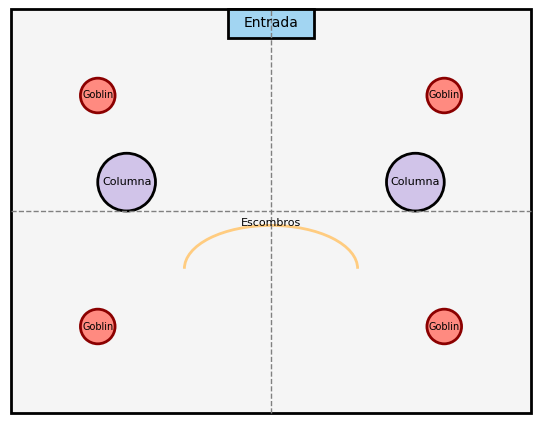
\includegraphics[keepaspectratio]{Figure_1.png}}

\textbf{El contorno del vestíbulo:} Con un rectángulo de fondo.

\textbf{La entrada principal:} Señalada en la parte superior central.

\textbf{Columnas (cobertura):} Dibujadas como círculos en posiciones
estratégicas.

\textbf{Posiciones de los goblins:} Indicadas por círculos de color
distintivo.

\textbf{Elementos del entorno:} Líneas y curvas para representar muros
derrumbados o barreras.

\subsection{Encuentro 2: El Laberinto de
Trampas}\label{encuentro-2-el-laberinto-de-trampas}

\textbf{Objetivo:} Poner a prueba las habilidades de percepción,
investigación y destreza para sortear trampas y acertijos.

\textbf{Ambiente:} Un pasillo laberíntico con mecanismos ocultos,
trampas mecánicas y elementos interactivos (palancas, placas de
presión).

\textbf{Desafíos}

\begin{itemize}
\tightlist
\item
  Trampas activadas por el peso o el movimiento, obligando a los
  jugadores a realizar tiradas de Destreza y Percepción.
\item
  Un enigma o mecanismo que, al resolverse correctamente, desactiva
  parte de las trampas o abre un acceso seguro.
\end{itemize}

\textbf{Dinámica:} Incentivar el uso de habilidades no combativas y la
coordinación para que algunos personajes vigilen mientras otros exploran
o desactivan las trampas.

\subsubsection{Objetivo}\label{objetivo-1}

Este encuentro está diseñado para poner a prueba las habilidades de
percepción, destreza y coordinación de los jugadores, obligándolos a
sortear trampas mecánicas y resolver un enigma para avanzar sin activar
peligros mayores. Se destaca la importancia de la observación y la
cooperación para desactivar mecanismos y encontrar rutas seguras.

\subsubsection{Ambientación y
narrativa}\label{ambientaciuxf3n-y-narrativa-1}

Los personajes se adentran en un pasillo laberíntico y oscuro, en el que
el suelo, las paredes y el techo muestran signos de deterioro. A lo
largo del recorrido, varios mecanismos ocultos y trampas esperan ser
descubiertos. Entre ellos, unas placas de presión, pinchos ocultos y
palancas que pueden modificar el entorno para desactivar o activar
trampas. \emph{``El aire se vuelve más frío y tenso al internarse en
este corredor abandonado. Las sombras se alargan y, en cada esquina,
parece haber algo fuera de lugar. Una serie de inscripciones y
mecanismos en las paredes insinúan que el camino es tan traicionero como
enigmático.}

\subsubsection{Desafíos y Mecánicas}\label{desafuxedos-y-mecuxe1nicas}

\textbf{Trampas activas:}

\begin{itemize}
\tightlist
\item
  Placas de presión en el suelo que al pisarlas pueden activar una
  lluvia de dardos o hacer caer pinchos.
\item
  Trampas ocultas en las paredes, detectables con tiradas de Percepción
  o Investigación.
\end{itemize}

\textbf{Enigma mecánico:} Una palanca o serie de interruptores que, al
activarse en el orden correcto, desactiva parte de las trampas y abre un
pasaje seguro.

\textbf{Zona segura:} Un breve espacio en el laberinto que permite a los
jugadores reagruparse y planificar su siguiente movimiento, fomentando
la comunicación y la estrategia.

\subsubsection{Dinámica del
Encuentro}\label{dinuxe1mica-del-encuentro-1}

\textbf{Exploración Cautelosa:} Los personajes deberán avanzar despacio,
utilizando habilidades de Percepción e Investigación para identificar
trampas antes de activarlas.

\textbf{Resolución de Enigma:} Al encontrar una serie de palancas o
interruptores, se les presentará un enigma (por ejemplo, basarse en
inscripciones antiguas o patrones en el entorno) que, al resolverse,
desactiva las trampas más letales.

\textbf{Coordinación en Movimiento:} La disposición del laberinto
favorecerá que algunos personajes se adelanten para comprobar la
seguridad, mientras otros vigilan o se posicionan para ayudar a
desactivar trampas en grupo.

\subsubsection{Recompensas y
Aprendizajes}\label{recompensas-y-aprendizajes-1}

\textbf{Importancia de la Percepción:} Los jugadores aprenderán a
valorar las tiradas de Percepción e Investigación para evitar daños y
encontrar pistas.

\textbf{Resolución de Problemas:} La necesidad de resolver un enigma
refuerza el juego en equipo y la aplicación creativa de habilidades.

\textbf{Gestión del Riesgo:} La planificación cuidadosa y el movimiento
coordinado se vuelven esenciales para superar el recorrido sin caer en
trampas fatales.

\subsection{Mapa Esquemático del Laberinto de
Trampas}\label{mapa-esquemuxe1tico-del-laberinto-de-trampas}

\pandocbounded{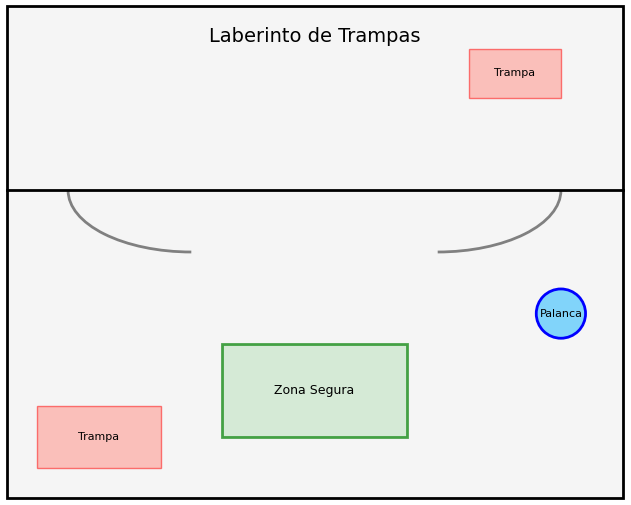
\includegraphics[keepaspectratio]{Figure_2.png}}

\textbf{Contorno del Laberinto:} Un gran rectángulo delimita el área del
laberinto, representando las paredes exteriores.

\textbf{Camino Principal y Giros:} La línea central y las curvas
(dibujadas con arcos) simulan el recorrido laberíntico que los
personajes deben explorar.

\textbf{Trampas:} Las áreas en color rojo (con transparencia) indican
zonas de riesgo, como placas de presión o trampas mecánicas.

\textbf{Zona Segura:} Un área marcada en verde pálido permite a los
jugadores reagruparse y planificar sus movimientos.

\textbf{Elemento Interactivo:} Una palanca en color azul que simboliza
el enigma mecánico que, al resolverse, desactiva algunas trampas.

\subsection{Encuentro 3: La emboscada de las
sombras}\label{encuentro-3-la-emboscada-de-las-sombras}

\textbf{Objetivo:} Enfatizar la importancia del sigilo, la detección y
el uso de la iluminación y el terreno a favor propio.

\subsubsection{Ambientación y
Enemigos}\label{ambientaciuxf3n-y-enemigos-1}

\textbf{Ambiente:} Un corredor oscuro iluminado solo por antorchas
dispersas, con zonas de sombra donde se ocultan los peligros.

\textbf{Enemigos:} Criaturas etéreas o espectros que se mueven
silenciosamente, aprovechando la oscuridad para atacar por sorpresa.

\textbf{Dinámica:}

\begin{itemize}
\tightlist
\item
  Permitir tiradas de Sigilo, Percepción e Investigación para que los PJ
  descubran los patrones de ataque y la posición oculta de los enemigos.
\item
  Incentivar el uso de hechizos o habilidades que generen luz o revelen
  lo oculto, evidenciando cómo el entorno puede volverse una ventaja
  táctica.
\end{itemize}

\subsubsection{Objetivo}\label{objetivo-2}

En este encuentro, los personajes se adentran en un corredor oscuro
donde la iluminación es escasa y la mayoría del espacio está sumido en
sombras. El objetivo es enfatizar la importancia del sigilo, la
percepción y el uso estratégico del entorno. Los jugadores deberán hacer
tiradas de Sigilo y Percepción para detectar a los enemigos espectrales,
que se ocultan en áreas de sombra, y utilizar la luz (por ejemplo,
antorchas o hechizos) para disipar la oscuridad y revelar sus
posiciones.

\subsubsection{Ambientación y
narrativa}\label{ambientaciuxf3n-y-narrativa-2}

El grupo avanza por un pasillo de la torre donde el ambiente se torna
inquietante. La única fuente de luz proviene de algunas antorchas
dispersas en el corredor, generando manchas de luminosidad que
contrastan fuertemente con las zonas en completa penumbra. En estas
sombras, se esconden espectros que aprovechan la oscuridad para emboscar
a los aventureros. La tensión aumenta mientras cada paso podría revelar
un peligro oculto.

\emph{``La penumbra se espesa a medida que avanzan por el corredor.
Apenas unos haces de luz de las antorchas cortan la oscuridad, revelando
formas vagamente humanas que se deslizan entre las sombras. ¿Serán
capaces de descubrir la posición de estos espectros antes de que sus
ataques les sorprendan?''}

\subsubsection{Enemigos}\label{enemigos-1}

\textbf{Espectros:}

\begin{itemize}
\tightlist
\item
  Apariencia fantasmal, difuminados y etéreos.
\item
  Se camuflan en las zonas de sombra, volviéndose difíciles de detectar
  a simple vista.
\item
  Vulnerables a la luz y a ataques mágicos. El conjuro Sanación no los
  cura, sino que los hiere mucho.
\end{itemize}

\subsubsection{Dinámica del
Encuentro}\label{dinuxe1mica-del-encuentro-2}

\textbf{Exploración en la oscuridad:} los personajes deberán avanzar con
cautela, utilizando tiradas de Percepción y Sigilo para identificar las
áreas donde se ocultan los espectros.

\textbf{Camina por la sombra:} se fomentará el uso de antorchas,
hechizos de luz u otros recursos que puedan iluminar el entorno,
revelando temporalmente a los enemigos ocultos.

\textbf{Ataques Sorpresa:} los espectros realizarán emboscadas
aprovechando la oscuridad, lo que obligará a los jugadores a adaptarse
rápidamente y a coordinarse para evitar ser superados.

\subsubsection{Recompensas y
Aprendizajes}\label{recompensas-y-aprendizajes-2}

\textbf{Valoración de la Percepción:} la necesidad de identificar
amenazas ocultas refuerza la importancia de las tiradas de Percepción.

\textbf{Uso Táctico de la Luz:} los jugadores aprenderán a utilizar
elementos ambientales (como antorchas o hechizos) para transformar el
terreno a su favor.

\textbf{Estrategia de Sigilo y Coordinación:} la combinación de
movimientos cautelosos y acciones coordinadas será clave para superar la
emboscada.

\subsection{Mapa del corredor oscuro}\label{mapa-del-corredor-oscuro}

\pandocbounded{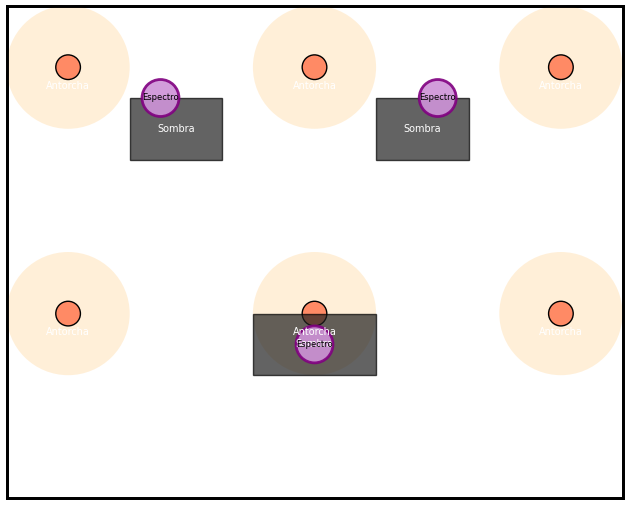
\includegraphics[keepaspectratio]{Figure_3.png}}

\textbf{Fondo oscuro:} El corredor está en penumbra, aunque en el mapa
para imprimir sea blanco.

\textbf{Antorchas y áreas iluminadas:} Se ubican en puntos estratégicos
para evidenciar cómo la luz disipa la oscuridad en áreas limitadas.

\textbf{Zonas de sombra:} Las áreas en negro intenso indican lugares
donde los espectros se ocultan, obligando a los jugadores a actuar con
cautela.

\textbf{Espectros:} Están marcados con círculos de tono púrpura,
representando enemigos que se aprovechan de la oscuridad para emboscar.

\subsection{Encuentro 4: duelo
táctico}\label{encuentro-4-duelo-tuxe1ctico}

\textbf{Objetivo:} Profundizar en la coordinación y la adaptación
táctica, utilizando el terreno y la combinación de habilidades y equipo.

\subsubsection{\texorpdfstring{\textbf{Ambientación y
enemigos}}{Ambientación y enemigos}}\label{ambientaciuxf3n-y-enemigos-2}

\textbf{Ambiente:} Una sala amplia con estructuras colapsadas,
plataformas elevadas y zonas que obligan a maniobras precisas.

\textbf{Enemigos:} Un grupo de mercenarios o esqueletos reanimados
organizados en formaciones, que se adaptan rápidamente al flujo del
combate.

\paragraph{\texorpdfstring{\textbf{Dinámica}}{Dinámica}}\label{dinuxe1mica}

Enfrentar a los jugadores a un combate dinámico donde cada posición y
movimiento cuente.

Permitir que algunas áreas ofrezcan ventajas (como coberturas o puntos
elevados) para ataques a distancia, obligando a que el grupo se coordine
y aproveche el terreno para flanquear a los enemigos.

Posibilitar el ajuste del equipo entre enfrentamientos, permitiendo a
los jugadores cambiar tácticas o preparar conjuros específicos en
función de las debilidades observadas en los oponentes.

\subsubsection{Objetivo}\label{objetivo-3}

El propósito de este encuentro es desafiar a los personajes a coordinar
sus movimientos y acciones en un entorno dinámico. La sala cuenta con
zonas elevadas, obstáculos derrumbados y áreas que obligan a maniobras
precisas. Los jugadores deberán usar el terreno a su favor para
flanquear a los enemigos, protegerse de ataques coordinados y adaptarse
rápidamente a los cambios del combate.

\subsubsection{Ambientación y
narrativa}\label{ambientaciuxf3n-y-narrativa-3}

Los aventureros se adentran en una sala amplia, antiguamente un gran
salón o vestíbulo, que ahora se encuentra parcialmente derrumbada.
Columnas caídas, muros agrietados y plataformas elevadas se intercalan
en el espacio, creando áreas de cobertura y puntos estratégicos. En este
ambiente caótico, un grupo de mercenarios o esqueletos reanimados se
dispone en formaciones, listos para explotar cualquier debilidad en la
coordinación de los PJ.

\emph{``Al ingresar al gran salón, notáis que el lugar parece haber sido
testigo de épicas batallas pasadas. Columnas derrumbadas y escombros se
mezclan con secciones aún en pie, ofreciendo oportunidades para moverse
y atacar desde posiciones inesperadas. Los enemigos, organizados y
letales, se mueven con rapidez, obligándoos a planificar cada acción con
precisión.''}

\subsubsection{Enemigos y dinámica de
combate}\label{enemigos-y-dinuxe1mica-de-combate}

\textbf{Enemigos:} un grupo de mercenarios o esqueletos reanimados,
organizados en formaciones.

\paragraph{Dinámica}\label{dinuxe1mica-1}

\textbf{Cobertura y Obstáculos:} el entorno ofrece numerosas coberturas:
escombros, columnas caídas y plataformas elevadas que deben ser
aprovechadas para protegerse o flanquear.

\textbf{Movilidad y Coordinación:} el combate se vuelve fluido,
requiriendo constantes movimientos para evitar quedar expuestos.

\textbf{Adaptación del Terreno:} algunos obstáculos pueden moverse o
derrumbarse tras ciertos impactos, cambiando la configuración del campo
de batalla en pleno combate.

\subsubsection{Recompensas y
Aprendizajes}\label{recompensas-y-aprendizajes-3}

\textbf{Coordinación de equipo:} Los jugadores deberán comunicarse y
coordinar sus movimientos para maximizar el uso del terreno.

\textbf{Adaptación táctica:} Se enfatiza la importancia de ajustar
estrategias en tiempo real, aprovechando las coberturas y anticipando el
movimiento del enemigo.

\textbf{Uso del entorno:} Aprenderán a identificar puntos estratégicos
que otorgan ventajas ofensivas y defensivas, como plataformas elevadas o
barreras naturales.

\subsection{Mapa del Gran Salón}\label{mapa-del-gran-saluxf3n}

\pandocbounded{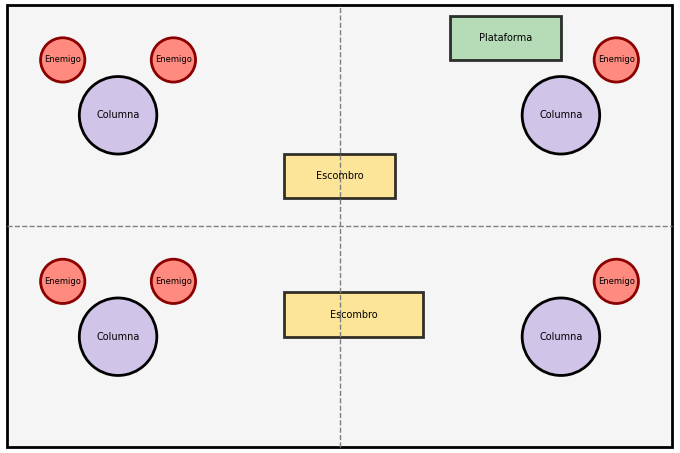
\includegraphics[keepaspectratio]{Figure_4.png}}

\textbf{Contorno del Gran Salón:} Representado por un gran rectángulo,
define el área del combate.

\textbf{Obstáculos Internos:}

\begin{itemize}
\tightlist
\item
  \textbf{Columnas Derrumbadas:} Creadas como círculos, ofrecen
  cobertura y se sitúan en posiciones estratégicas.
\item
  \textbf{Escombros:} Rectángulos que simulan áreas bloqueadas o que
  pueden servir de cobertura.
\item
  \textbf{Plataforma Elevada:} Una zona diferenciada que otorga ventaja
  para ataques a distancia o para observar el campo de batalla.
\end{itemize}

\textbf{Líneas Divisorias:} Las líneas punteadas muestran muros
derrumbados o zonas que separan áreas, obligando a los jugadores a
adaptarse en sus movimientos.

\textbf{Posiciones de los Enemigos:} Los círculos rojos indican dónde se
encuentran inicialmente los adversarios, promoviendo la necesidad de
flanquear o coordinar ataques.

\subsection{Encuentro 5: El Enfrentamiento del Maestro de la Estrategia
(Jefe
Final)}\label{encuentro-5-el-enfrentamiento-del-maestro-de-la-estrategia-jefe-final}

\textbf{Objetivo:} Culminar la sesión con un desafío complejo que
combine habilidades, estrategia en equipo y el aprovechamiento de
debilidades específicas.

\subsubsection{Ambientación y Enemigo}\label{ambientaciuxf3n-y-enemigo}

\textbf{Ambiente:} Una gran sala del trono con estructuras colapsadas,
zonas de cobertura y elementos interactivos (por ejemplo, mecanismos que
activen trampas a favor de los jugadores o en detrimento del jefe).

\textbf{Enemigo:} El Maestro de la Estrategia, un jefe con múltiples
fases (por ejemplo, un caballero espectral o un hechicero caído) que usa
tanto ataques a distancia como cuerpo a cuerpo.

\subsubsection{Objetivo}\label{objetivo-4}

El objetivo de este encuentro es desafiar a los personajes con un jefe
que evoluciona durante la batalla. El Maestro de la Estrategia (por
ejemplo, un caballero espectral o un hechicero caído) posee varias
fases:

\textbf{Fase Inicial:} Defiende sus ataques combinados, presentando un
desafío moderado.

\textbf{Fase de Adaptación:} Al recibir cierto porcentaje de daño,
activa habilidades especiales o convoca esbirros, dificultando el
combate y ofreciendo pistas sobre su debilidad.

\textbf{Fase Final:} Durante un breve lapso, se expone una
vulnerabilidad crítica que los jugadores deben explotar de manera
coordinada para lograr la victoria.

\subsubsection{Ambientación y
narrativa}\label{ambientaciuxf3n-y-narrativa-4}

El enfrentamiento tiene lugar en una gran sala del trono, antigua y
majestuosa, pero ahora en ruinas. La sala presenta estructuras
colapsadas, escombros y niveles de altura que permiten esconderse o
posicionarse estratégicamente.

\emph{``La gran sala del trono, que en su día albergó la gloria de un
imperio, ahora es el escenario de un combate épico. El Maestro de la
Estrategia se alza en el centro, rodeado de escombros y trampas
mecánicas, mientras sus ataques y convocatorias de esbirros ponen a
prueba la coordinación y el valor de los aventureros. En un parpadeo, se
abre una oportunidad: una parte de su armadura brilla con una luz
extraña. Este es el momento para unir fuerzas y atacar.''}

\subsubsection{Dinámica del
Encuentro}\label{dinuxe1mica-del-encuentro-3}

\textbf{Fase Inicial}

\begin{itemize}
\tightlist
\item
  El jefe utiliza ataques mixtos (a distancia y cuerpo a cuerpo) y
  mantiene una defensa moderada.
\item
  Los jugadores deben aprender sus patrones de ataque y posicionarse
  estratégicamente aprovechando el entorno (columnas, escombros, niveles
  de altura).
\end{itemize}

\textbf{Fase de Adaptación}

\begin{itemize}
\tightlist
\item
  Al alcanzar un umbral de vida, el jefe activa una habilidad especial
  (por ejemplo, un aura que reduce el daño o convoca esbirros
  temporales).
\item
  Se ofrecen indicios visuales de una vulnerabilidad: puede ser una
  parte de su armadura que se ilumina brevemente o un movimiento
  errático que deja un punto expuesto.
\end{itemize}

\textbf{Fase Final}

\begin{itemize}
\tightlist
\item
  La vulnerabilidad se revela durante un corto periodo, donde la
  coordinación y el ataque concentrado son decisivos.
\item
  Los jugadores tienen que aprovechar todos los recursos adquiridos en
  encuentros previos (uso del entorno, habilidades de percepción y
  coordinación en equipo).
\end{itemize}

\subsubsection{Recompensas y
aprendizajes}\label{recompensas-y-aprendizajes-4}

\textbf{Coordinación y comunicación:} La necesidad de coordinar ataques
y defenderse simultáneamente enfatiza el trabajo en equipo.

\textbf{Adaptabilidad táctica:} Los jugadores aprenderán a adaptarse a
cambios rápidos en la situación de combate, analizando pistas y
ajustando estrategias en tiempo real.

\textbf{Uso Integral del entorno:} La sala del trono, con sus múltiples
niveles y obstáculos, ofrece oportunidades para posicionarse, cubrirse y
atacar desde ángulos inesperados.

\subsection{Mapa de la Sala del Trono (encuentro
final)}\label{mapa-de-la-sala-del-trono-encuentro-final}

\pandocbounded{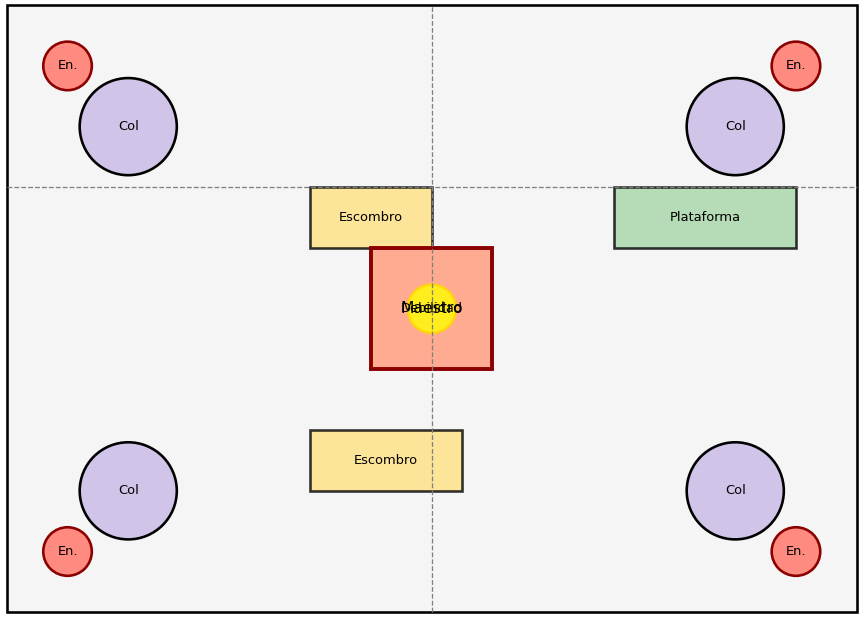
\includegraphics[keepaspectratio]{Figure_5.png}}

\textbf{Contorno de la Sala:} Un gran rectángulo define el espacio del
combate, simulando las paredes y la estructura de la antigua sala del
trono.

\textbf{Columnas y Escombros:} Se representan con círculos y rectángulos
que actúan como cobertura o barreras estratégicas.

\textbf{Plataforma Elevada:} una zona diferenciada que ofrece ventajas
tácticas, ideal para ataques a distancia o para tener una mejor visión
del campo.

\textbf{El jefe final:} ubicado en el centro, se representa con un
rectángulo y se le añade un círculo indicador (vulnerabilidad) que
señala el momento crítico de la batalla.

\textbf{Esbirros y muros internos:} líneas punteadas y posiciones de
enemigos secundarios complementan la dinámica del combate, obligando a
los jugadores a gestionar múltiples amenazas y aprovechar el entorno.

\section{Enemigos}\label{enemigos-2}

\subsection{1. Guardián goblin}\label{guardiuxe1n-goblin}

\emph{(Encuentro 1: El Umbral de la Torre)}

\textbf{Descripción:} Estos goblins actúan como guardianes menores en la
entrada de la torre. Son rápidos, escurridizos y aprovechan el terreno
en ruinas para emboscar a los aventureros.

\textbf{Estadísticas:}

\begin{itemize}
\tightlist
\item
  \textbf{Clase de Armadura (CA):} 15 (ligera armadura, aprovechando su
  agilidad)
\item
  \textbf{Puntos de Golpe (PG):} 7 (2d6)
\item
  \textbf{Velocidad:} 30 pies
\end{itemize}

\textbf{Atributos:}

\begin{longtable}[]{@{}cccccc@{}}
\toprule\noalign{}
FUE & DES & CON & INT & SAB & CAR \\
\midrule\noalign{}
\endhead
\bottomrule\noalign{}
\endlastfoot
8 (-1) & 14 (+2) & 10 & 10 & 8 (-1) & 8 (-1) \\
\end{longtable}

\textbf{Habilidades:} Sigilo +6, Percepción +2

\textbf{Sentidos:} Visión en la oscuridad 60 pies; Percepción pasiva 11

\textbf{Idiomas:} Común, Goblin

\textbf{Ataques:}

\begin{itemize}
\tightlist
\item
  \textbf{Cimitarra:}

  \begin{itemize}
  \tightlist
  \item
    \emph{Ataque cuerpo a cuerpo:} +4 al golpe, alcance 5 pies, un
    objetivo.
  \item
    \emph{Impacto:} 5 (1d6 + 2) daño cortante.
  \end{itemize}
\item
  \textbf{Arco Corto:}

  \begin{itemize}
  \tightlist
  \item
    \emph{Ataque a distancia:} +4 al golpe, alcance 80/320 pies, un
    objetivo.
  \item
    \emph{Impacto:} 5 (1d6 + 2) daño perforante.
  \end{itemize}
\end{itemize}

\textbf{Habilidad Especial:}

\begin{itemize}
\tightlist
\item
  \textbf{Escape Ágil:} Puede tomar la acción de Desenganche o
  Esconderse como acción adicional en cada uno de sus turnos, lo que le
  permite reposicionarse rápidamente y aprovechar su entorno.
\end{itemize}

\subsection{2. Trampas del laberinto}\label{trampas-del-laberinto}

\emph{(Encuentro 2: El Laberinto de Trampas)}

Aunque no son ``enemigos vivos'', las trampas representan amenazas
letales. Aquí dos ejemplos de trampas mecánicas:

\subsubsection{a) Trampa de placas de presión (Dardos
Ocultos)}\label{a-trampa-de-placas-de-presiuxf3n-dardos-ocultos}

\begin{itemize}
\tightlist
\item
  \textbf{Detección:} Tirada de Percepción DC 13 para notar
  irregularidades en el suelo.
\item
  \textbf{Desarme:} Prueba de Herramientas de ladrón o Destreza DC 13.
\item
  \textbf{Efecto:}

  \begin{itemize}
  \tightlist
  \item
    Al activarse, dispara dardos desde las paredes.
  \item
    Cada criatura en un área de 5×5 pies debe realizar una tirada de
    Destreza DC 13.
  \item
    En fallo, recibe 2d6 de daño perforante; con éxito, la mitad.
  \end{itemize}
\end{itemize}

\subsubsection{b) Trampa de pinchos}\label{b-trampa-de-pinchos}

\begin{itemize}
\tightlist
\item
  \textbf{Detección:} Tirada de Percepción DC 15 para descubrir la
  sección debilitada del suelo.
\item
  \textbf{Desarme:} Prueba de Destreza DC 15.
\item
  \textbf{Efecto:}

  \begin{itemize}
  \tightlist
  \item
    Al activarse, el suelo se abre y revela pinchos afilados.
  \item
    Las criaturas en el área deben hacer una tirada de Destreza DC 15.
  \item
    En fallo, reciben 3d6 de daño perforante; con éxito, la mitad.
  \end{itemize}
\end{itemize}

\subsection{3. Espectro Sombrío}\label{espectro-sombruxedo}

\emph{(Encuentro 3: La Emboscada de las Sombras)}

\textbf{Descripción:}\\
Seres etéreos que se ocultan en la penumbra, emboscando a los
personajes. Su forma difusa y su vínculo con la oscuridad les hacen
difíciles de combatir, salvo que se expongan a luz intensa.

\textbf{Estadísticas:}

\begin{itemize}
\tightlist
\item
  \textbf{CA:} 12
\item
  \textbf{PG:} 22 (5d8)
\item
  \textbf{Velocidad:} 0 pies (terrestre); Vuelo 50 pies (flotando)
\end{itemize}

\textbf{Atributos:}

\begin{longtable}[]{@{}cccccc@{}}
\toprule\noalign{}
FUE & DES & CON & INT & SAB & CAR \\
\midrule\noalign{}
\endhead
\bottomrule\noalign{}
\endlastfoot
6 (-2) & 14 (+2) & 10 & 10 & 12 (+1) & 17 (+3) \\
\end{longtable}

\textbf{Habilidades y Sentidos:}

\begin{itemize}
\tightlist
\item
  \textbf{Resistencias:}

  \begin{itemize}
  \tightlist
  \item
    Resiste daños de armas no mágicas (bludgeoning, perforante y
    cortante).
  \item
    Inmunidad al daño necrótico y al veneno; inmunidades a condiciones
    (envenenado, paralizado, etc.).
  \end{itemize}
\item
  \textbf{Sentidos:} Visión en la oscuridad 60 pies; Percepción pasiva
  11
\item
  \textbf{Idiomas:} Entiende los idiomas que conocía en vida, pero no
  puede hablar.
\item
  \textbf{Desafío:} 1 (200 XP)
\end{itemize}

\textbf{Ataque: Drenaje Vital}

\begin{itemize}
\tightlist
\item
  \emph{Ataque cuerpo a cuerpo:} +4 al golpe, alcance 5 pies, un
  objetivo.
\item
  \emph{Impacto:} 10 (2d6 + 3) daño necrótico.
\item
  \emph{Efecto Adicional:} La criatura impactada debe superar una
  salvación de Constitución DC 10 o reducirse sus puntos de golpe
  máximos en la cantidad de daño infligido.
\end{itemize}

\textbf{Habilidad Adicional:}

\begin{itemize}
\tightlist
\item
  \textbf{Vulnerabilidad a la Luz:} Si se expone a luz brillante (por
  ejemplo, mediante un hechizo o una fuente de luz intensa), el espectro
  recibe 1d6 de daño adicional por cada ataque exitoso que lo impacte.
\end{itemize}

\subsection{4. Mercenario Esquelético}\label{mercenario-esqueluxe9tico}

\emph{(Encuentro 4: El Duelo Táctico)}

\textbf{Descripción:}\\
Estos combatientes reanimados son soldados caídos que han vuelto a la
lucha. Son menos resistentes que otros no-muertos, pero su coordinación
táctica los hace peligrosos en grupo.

\textbf{Estadísticas:}

\begin{itemize}
\tightlist
\item
  \textbf{CA:} 13 (Armadura natural)
\item
  \textbf{PG:} 13 (2d8 + 4)
\item
  \textbf{Velocidad:} 30 pies
\end{itemize}

\textbf{Atributos:}

\begin{longtable}[]{@{}cccccc@{}}
\toprule\noalign{}
FUE & DES & CON & INT & SAB & CAR \\
\midrule\noalign{}
\endhead
\bottomrule\noalign{}
\endlastfoot
10 & 14 (+2) & 15 (+2) & 6 (-2) & 8 (-1) & 5 (-3) \\
\end{longtable}

\textbf{Habilidades y Sentidos:}

\begin{itemize}
\tightlist
\item
  \textbf{Vulnerabilidad:} Reciben daño contundente adicional.
\item
  \textbf{Ataques:}

  \begin{itemize}
  \tightlist
  \item
    \textbf{Espada Corta:}

    \begin{itemize}
    \tightlist
    \item
      \emph{Ataque cuerpo a cuerpo:} +4 al golpe, alcance 5 pies.
    \item
      \emph{Impacto:} 1d6 + 2 daño cortante.
    \end{itemize}
  \item
    \textbf{Arco Corto:}

    \begin{itemize}
    \tightlist
    \item
      \emph{Ataque a distancia:} +4 al golpe, alcance 80/320 pies.
    \item
      \emph{Impacto:} 1d6 + 2 daño perforante.
    \end{itemize}
  \end{itemize}
\item
  \textbf{Habilidad Especial -- Golpe Coordinado:}

  \begin{itemize}
  \tightlist
  \item
    Si al menos otro mercenario esquelético está adyacente al mismo
    objetivo, este ataque se realiza con ventaja.
  \end{itemize}
\end{itemize}

\subsection{5. Maestro de la Estrategia}\label{maestro-de-la-estrategia}

\emph{(Encuentro Final: El Enfrentamiento del Jefe)}

\textbf{Descripción:} El Maestro de la Estrategia es un enemigo
formidable que ha perfeccionado el arte de la batalla. Con múltiples
fases en el combate, desafía a los aventureros a adaptarse y coordinarse
para descubrir su punto débil.

\textbf{Estadísticas:}

\begin{itemize}
\tightlist
\item
  \textbf{CA:} 17 (en fase inicial, usando cota de malla y escudo)
\item
  \textbf{PG:} 150 (20d8 + 60)
\item
  \textbf{Velocidad:} 30 pies
\end{itemize}

\textbf{Atributos:}

\begin{longtable}[]{@{}cccccc@{}}
\toprule\noalign{}
FUE & DES & CON & INT & SAB & CAR \\
\midrule\noalign{}
\endhead
\bottomrule\noalign{}
\endlastfoot
16 (+3) & 12 (+1) & 16 (+3) & 14 (+2) & 12 (+1) & 18 (+4) \\
\end{longtable}

\textbf{Habilidades y Sentidos:}

\begin{itemize}
\tightlist
\item
  \textbf{Salvaciones:} Constitución +7, Sabiduría +5, Carisma +8
\item
  \textbf{Habilidades:} Percepción +5, Perspicacia +5
\item
  \textbf{Sentidos:} Percepción pasiva 15
\item
  \textbf{Idiomas:} Común (y otros, según el trasfondo)
\item
  \textbf{Desafío:} Aproximadamente 8--9 (ajustable según la experiencia
  deseada)
\end{itemize}

\textbf{Acciones:}

\begin{itemize}
\tightlist
\item
  \textbf{Multiataque:} Realiza tres ataques en su turno (dos con su
  espada larga y uno con un proyectil arcano).
\item
  \textbf{Espada Larga:}

  \begin{itemize}
  \tightlist
  \item
    \emph{Ataque cuerpo a cuerpo:} +7 al golpe, alcance 5 pies.
  \item
    \emph{Impacto:} 9 (1d8 + 5) daño cortante (1d10 + 5 si se usa a dos
    manos).
  \end{itemize}
\item
  \textbf{Proyectil Arcano:}

  \begin{itemize}
  \tightlist
  \item
    \emph{Ataque a distancia:} +6 al golpe, alcance 60 pies.
  \item
    \emph{Impacto:} 10 (2d6 + 3) daño de fuerza.
  \end{itemize}
\end{itemize}

\textbf{Habilidad Especial -- Táctica Inspiradora:}

\begin{itemize}
\tightlist
\item
  Una vez cada corto descanso, puede usar una acción adicional para
  inspirar a sus aliados en un radio de 30 pies, otorgándoles ventaja en
  los ataques hasta el inicio de su siguiente turno.
\end{itemize}

\textbf{Fase de Cambio (Segunda Fase):} Cuando sus puntos de golpe caen
a 75 o menos, el Maestro entra en una fase más agresiva:

\begin{itemize}
\tightlist
\item
  \textbf{Pérdida del Escudo:} Su CA baja a 15.
\item
  \textbf{Ataque Adicional:} Gana un ataque extra en su turno.
\item
  \textbf{Indicador de Vulnerabilidad:} Durante 1 ronda, su punto débil
  (señalado en el mapa como ``Debilidad'') queda expuesto; los ataques
  que impacten esa zona infligen 1d8 de daño adicional.
\end{itemize}

\textbf{Acciones Legendarias (Opcional):} Puede tomar 2 acciones
legendarias al final del turno de otro enemigo, eligiendo entre:

\begin{itemize}
\tightlist
\item
  \textbf{Movimiento:} Desplazarse hasta la mitad de su velocidad sin
  provocar ataques de oportunidad.
\item
  \textbf{Ataque Extra:} Realizar un ataque con su espada larga.
\end{itemize}

\textbf{Legendary Resistance:} 1 vez al día para evitar quedar
incapacitado por un efecto.

\textbf{Esbirros del Maestro:} Durante el encuentro final, es posible
que aparezcan esbirros (como mercenarios esqueléticos) que utilicen las
mismas estadísticas que los Mercenarios Esqueléticos descritos, ayudando
a complementar la dificultad del combate y obligando a los jugadores a
gestionar múltiples amenazas.

\section{Personajes Jugadores (PJ)}\label{personajes-jugadores-pj}

\subsection{1. Thorin ``El Férreo'' -- Guerrero (Battle
Master)}\label{thorin-el-fuxe9rreo-guerrero-battle-master}

\textbf{Descripción:} Tanque y estratega cuerpo a cuerpo, capaz de
controlar el campo de batalla mediante maniobras tácticas.

\begin{longtable}[]{@{}cccccc@{}}
\toprule\noalign{}
FUE & DES & CON & INT & SAB & CAR \\
\midrule\noalign{}
\endhead
\bottomrule\noalign{}
\endlastfoot
16 (+3) & 14 (+2) & 16 (+3) & 10 & 12 (+1) & 10 \\
\end{longtable}

\textbf{PG:} 50

\textbf{CA:} 18 (Armadura de placas o cota de malla + escudo)

\textbf{Equipo y Armas:}

\begin{itemize}
\tightlist
\item
  \textbf{Armadura pesada:} Cota de malla o placas
\item
  \textbf{Escudo:} +2 a CA
\item
  \textbf{Arma principal:} Espada larga (o gran espada, según
  preferencia)

  \begin{itemize}
  \tightlist
  \item
    \emph{Ataque:} +7; Daño: 1d8+3 (1d10+3 a dos manos)
  \end{itemize}
\item
  \textbf{Arma secundaria:} Dardo o hacha ligera para ataques a
  distancia
\item
  \textbf{Herramientas tácticas:} Dados de superioridad (maniobras como
  Trip Attack, Disarming Attack, Precision Attack)
\item
  \textbf{Equipo adicional:} Botiquín básico, cuaderno de estrategias y
  un mapa esquemático de la torre
\end{itemize}

\textbf{Habilidad Especial:}

\begin{itemize}
\tightlist
\item
  \textbf{Maniobras de Batalla:} Puede utilizar sus dados de
  superioridad para imponer efectos tácticos (desarmar, empujar, etc.) y
  coordinar sus ataques con precisión.
\end{itemize}

\subsection{2. Eldrin ``El Astuto'' -- Mago
(Evocador)}\label{eldrin-el-astuto-mago-evocador}

\textbf{Descripción:} Control del campo y daño a distancia mediante
magia, capaz de analizar y explotar las debilidades enemigas.

\begin{longtable}[]{@{}cccccc@{}}
\toprule\noalign{}
FUE & DES & CON & INT & SAB & CAR \\
\midrule\noalign{}
\endhead
\bottomrule\noalign{}
\endlastfoot
8 (-1) & 12 (+1) & 14 (+2) & 17 (+3) & 13 (+1) & 10 \\
\end{longtable}

\textbf{PG:} 30

\textbf{CA:} 12 (con armadura de mago o sin armadura; puede usar el
hechizo \emph{Escudo} en momentos críticos)

\textbf{Equipo y Armas:}

\begin{itemize}
\tightlist
\item
  \textbf{Arma:} Bastón o vara (sirve como foco arcano)
\item
  \textbf{Concentración en hechizos:}

  \begin{itemize}
  \tightlist
  \item
    \emph{Ataques y control:} \emph{Misil Mágico}, \emph{Rayo de
    Escarcha}
  \item
    \emph{Defensivos:} \emph{Escudo}, \emph{Armadura de Mago}
  \item
    \emph{Utilitarios y de movilidad:} \emph{Detectar Magia}, \emph{Paso
    Nebuloso}
  \end{itemize}
\item
  \textbf{Componentes:} Bolsa de componentes y su libro de hechizos
  (anotaciones de estrategias y tácticas)
\end{itemize}

\textbf{Habilidad Especial:}

\begin{itemize}
\tightlist
\item
  \textbf{Conocimiento Arcano:} Puede identificar debilidades mágicas o
  estructurales en enemigos y trampas, proporcionando información
  táctica al grupo.
\end{itemize}

\subsection{3. Lyra ``La Sombra'' -- Pícara (Arcane
Trickster)}\label{lyra-la-sombra-puxedcara-arcane-trickster}

\textbf{Rol:} Especialista en infiltración, desactivación de trampas y
ataques sorpresa. Su agilidad le permite aprovechar el entorno para
emboscar enemigos.

\begin{longtable}[]{@{}cccccc@{}}
\toprule\noalign{}
FUE & DES & CON & INT & SAB & CAR \\
\midrule\noalign{}
\endhead
\bottomrule\noalign{}
\endlastfoot
8 (-1) & 17 (+3) & 14 (+2) & 12 (+1) & 13 (+1) & 10 \\
\end{longtable}

\textbf{PG:} 35

\textbf{CA:} 15 (Armadura de cuero tachonado)

\textbf{Equipo y Armas:}

\begin{itemize}
\tightlist
\item
  \textbf{Arma principal:} Estoque o rapier

  \begin{itemize}
  \tightlist
  \item
    \emph{Ataque:} +7; Daño: 1d8+3 perforante
  \end{itemize}
\item
  \textbf{Arma a distancia:} Arco corto o ballestas ligeras

  \begin{itemize}
  \tightlist
  \item
    \emph{Ataque:} +7; Daño: 1d6+3 perforante
  \end{itemize}
\item
  \textbf{Herramientas:} Kit de ladrón (para desactivar trampas y abrir
  cerraduras)
\item
  \textbf{Complementos:} Capa o capa de elfo (para mejorar su sigilo) y
  polvos de distracción
\end{itemize}

\textbf{Habilidad Especial:}

\begin{itemize}
\tightlist
\item
  \textbf{Ataque Furtivo:} Si ataca a un enemigo que está distraído o
  flanqueado, añade daño extra.
\item
  \textbf{Maestría en Trampas:} Puede detectar y desactivar trampas con
  facilidad, clave en el Laberinto de Trampas.
\end{itemize}

\subsection{4. Kael ``El Justiciero'' -- Paladín (Juramento de la
Devoción)}\label{kael-el-justiciero-paladuxedn-juramento-de-la-devociuxf3n}

\textbf{Rol:} Combatiente frontal y sanador, que combina la lucha cuerpo
a cuerpo con poderes divinos para proteger y motivar al grupo.

\begin{longtable}[]{@{}cccccc@{}}
\toprule\noalign{}
FUE & DES & CON & INT & SAB & CAR \\
\midrule\noalign{}
\endhead
\bottomrule\noalign{}
\endlastfoot
16 (+3) & 10 & 14 (+2) & 10 & 12 (+1) & 16 (+3) \\
\end{longtable}

\textbf{PG:} 45

\textbf{CA:} 18 (Armadura completa y escudo)

\textbf{Equipo y Armas:}

\begin{itemize}
\tightlist
\item
  \textbf{Armadura:} Armadura completa
\item
  \textbf{Escudo:} +2 a CA
\item
  \textbf{Arma principal:} Espada larga o maza

  \begin{itemize}
  \tightlist
  \item
    \emph{Ataque:} +6; Daño: 1d8+3 contundente o cortante
  \end{itemize}
\item
  \textbf{Arma secundaria:} Jabalinas o ballesta ligera (para ataques a
  distancia)
\item
  \textbf{Equipo adicional:} Símbolo sagrado, pociones curativas y
  pergaminos de bendición
\item
  \textbf{Hechizos de Paladín:} \emph{Bendición}, \emph{Curar Heridas},
  \emph{Escudo de la Fe}, \emph{Golpe Divino}
\end{itemize}

\textbf{Habilidad Especial:}

\begin{itemize}
\tightlist
\item
  \textbf{Divina Inspiración:} Puede usar su aura para inspirar a sus
  aliados, otorgando ventajas en ataques o salvaciones, además de
  canalizar energía divina para infligir daño extra a los enemigos.
\end{itemize}

\subsection{5. Thalia ``La Furtiva'' --
Guardabosques}\label{thalia-la-furtiva-guardabosques}

\textbf{Rol:} Exploradora y rastreadora, experta en la supervivencia y
en el ataque a distancia, con un fuerte enfoque en la observación y la
movilidad.

\begin{longtable}[]{@{}cccccc@{}}
\toprule\noalign{}
FUE & DES & CON & INT & SAB & CAR \\
\midrule\noalign{}
\endhead
\bottomrule\noalign{}
\endlastfoot
10 & 16 (+3) & 14 (+2) & 10 & 16 (+3) & 8 (-1) \\
\end{longtable}

\textbf{PG:} 40

\textbf{CA:} 14--15 (Armadura de cuero tachonado o de cota de mallas
ligera)

\textbf{Equipo y Armas:}

\begin{itemize}
\tightlist
\item
  \textbf{Arma principal:} Arco largo

  \begin{itemize}
  \tightlist
  \item
    \emph{Ataque:} +7; Daño: 1d8+3 perforante
  \end{itemize}
\item
  \textbf{Armas cuerpo a cuerpo:} Dos espadas cortas o dagas

  \begin{itemize}
  \tightlist
  \item
    \emph{Ataque:} +7; Daño: 1d6+3 perforante
  \end{itemize}
\item
  \textbf{Equipo adicional:} Botiquín de supervivencia, kit de
  explorador, cuerdas y trampas rudimentarias
\item
  \textbf{Habilidades extras:} Conocimiento en rastreo, supervivencia y
  detección de trampas, además de algunos conjuros menores de
  guardabosques (como \emph{Salva de Flechas} o \emph{Paso Sin Rastro}).
\end{itemize}

\textbf{Habilidad Especial:}

\begin{itemize}
\tightlist
\item
  \textbf{Rastreadora Natural:} Tiene ventaja en tiradas de Sabiduría
  para detectar pistas, seguir rastros y anticipar emboscadas, lo cual
  es clave en los recorridos de la torre y en la detección de trampas.
\end{itemize}

\subsubsection{Cómo se integran en la
aventura}\label{cuxf3mo-se-integran-en-la-aventura}

Cada uno de estos personajes está pensado para aprovechar diferentes
aspectos de la aventura:

\textbf{Thorin y Kael} pueden encargarse de la línea frontal en combates
intensos (enfrentando guardianes, mercenarios y el jefe).

\textbf{Eldrin} ofrece control y explosiones mágicas, revelando
vulnerabilidades en los enemigos o trampas.

\textbf{Lyra} es ideal para la exploración sigilosa y la desactivación
de trampas en el Laberinto, además de emboscar a enemigos en el Umbral o
en emboscadas.

\textbf{Thalia} complementa la detección de peligros, el seguimiento de
movimientos enemigos y aporta potencia a distancia, siendo esencial para
emboscadas o para apoyar desde lejos.

La diversidad de roles obliga al grupo a colaborar: deberán coordinar
ataques, compartir información sobre trampas o debilidades y utilizar el
entorno a su favor. La combinación de fuerza bruta, magia, sigilo,
sanación y exploración garantiza que cada encuentro de la Torre del
Estratega se convierta en un reto táctico en el que todos tengan un
papel vital.

\end{document}
